\title{COM S 352 Homework 2}
\author{Alec Meyer}

\date{\today}

\documentclass[11pt]{article}
\usepackage{changepage}
\usepackage{graphicx}
\usepackage{amsmath}
\graphicspath{ {./images/} }
\newcommand\tab[1][1cm]{\hspace*{#1}}
\usepackage{amssymb}


\begin{document}
\maketitle


\section*{Question 1}
    First the operating system saves all data then transfers 
    control the the kernal. The kernel saves the context of 
    the old proccess in its PCB and then grabs the new process 
    and loads the saved data into the new process. Finally the 
    OS transfers control back to user mode.
\section*{Question 2}
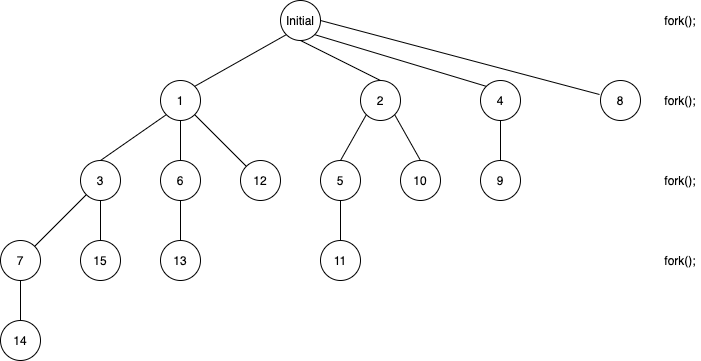
\includegraphics[scale=0.52]{COMS352HW2Q2}
16 total processes created 

\newpage
\section*{Question 3}
    The program executes, then runs into the \emph{fork()} function,
    where it creates a child process. This child process will enter 
    the \emph{else if} statement because its pid is 0 then it will
    hit the \emph{exec()} function. The \emph{exec()} function replaces
    the childs memory space with a new program, in this case it is
    \emph{ls}. Now that the child no longer exsists it will not reach 
    the line, \emph{printf("LINE J")}. However, if the \emph{exec()}
    function results in an error and memory is not replaced the
    child process will run the line \emph{printf("LINE J")}.
\section*{Question 4}
A: 0    \, \quad \qquad  //child\\
B: 2606 \qquad //child\\
C: 2606 \qquad //parent\\
D: 2603 \qquad //parent\\
\section*{Question 5}
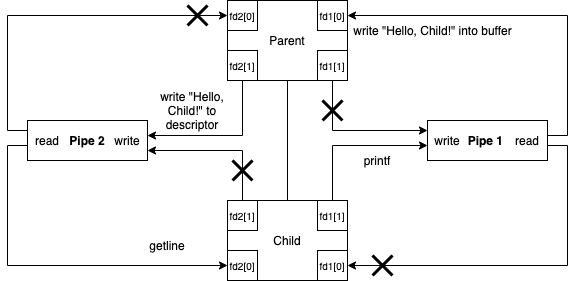
\includegraphics[scale=0.4]{COMS352HW2Q5.png}\\
The program starts with its initializations, \emph{int fd1[2]},
\emph{int fd2[2]}, and \emph{pid\_t pid = fork()} Then the child 
goes into the \emph{if(pid == 0)} block where it closes a read and
write descriptor then turns \emph{fd1[1]} into a \emph{printf} and 
\emph{fd2[0]} into 
a \emph{getline} using the \emph{dup2()} function. The child then
runs the \emph{execlp()} function and the child process terminates while
also allowing the parent to communicate between the two pipes.
The parent goes into the \emph{else} block and closes another read
and write then writes "Hello, Child!" to pipe 1, like mentioned before,
the \emph{execlp("cat", "cat", NULL)} allows the parent to read the 
message "Hello, Child!" from pipe 2 and save it in the buffer. The
program then prints out the buffer. 
\section*{Question 6}
    $\delta / (\delta + \sigma)$\\\\
    System A:\\
    $\delta$ = 20ms\\
    $\sigma$ = 1ms\\\\
    $20 / (20 + 1)$\\
    = 95.24\%\\\\
    System B:\\
    $\delta$ = 15ms\\
    $\sigma$ = 1ms\\\\
    $15 / (15 + 1)$\\
    =93.75\%

\section*{Question 7}
\begin{enumerate}
    \item \textbf{Running to Waiting}\\
        During an I/O or event wait, The process is going to enter a 
        waiting state because it is waiting for I/O input/output.
    \item \textbf{Waiting to Ready}\\
        After waiting for an I/O response (completion) it 
        will move to a ready state where it waits for 
        reassignment.
    \item \textbf{Running to Ready}\\
        The transition from running to ready will 
        occur when an interrupt is triggered. 
\end{enumerate}
\end{document}
